%% content.tex
%%


%% ===========================
\chapter{Umsetzung}
\label{ch:umsetzung}
%% ===========================

In diesem Kapitel wird auf die Implementierung der Konzepte eingegangen. Die Architektur wurde wie in der Konzeption beschrieben umgesetzt. Daher wird vielmehr auf die genauen Funktionsweisen und Prozesse eingegangen. Anhand von Klassendiagrammen wird in den ersten beiden Abschnitten die Struktur und Funktionsweise der Webprojekte erläutert. Weiterhin wird der ETL-Prozess und die Abfrageerzeugung detailliert beschrieben. Die Vorgänge die innerhalb einer Aktualisierung stattfinden werden in dem darauf folgenden Abschnitt behandelt. Abschließend wird der Aufbau der Oberfläche mit den damit verbundenen Designentscheidungen erläutert. 

%% ===========================
\section{Server-Webprojekt}
%% ===========================

Es handelt sich um ein Java-basiertes Eclipse-Webproject. Mithilfe der darin verwendeten Klassen wird die Struktur des Projektes erläutert. Abbildung \ref{umsetzung_klassendiagramm_server} zeigt das Klassendiagramm des Server-Webprojekt. Das Diagramm dient als Basis für die nachfolgenden Erläuterungen. 

Die H2-Datenbank wird im Embedded-Modus betrieben, was eine Instanziierung der Datenbank zur Laufzeit notwendig macht. Die Instanziierung erfolgt in der Klasse \textit{Database}. Das Attribut \textit{dataSource} stellt die H2-Datenbank in Form eines Objektes dar. Eine Verbindung zur Datenbank wird mithilfe der Methode \textit{getConnection()} aufgebaut. Diese Verbindung wird permanent offen gehalten, solang der Tomcat-Server läuft. Diese Verbindung wird mithilfe des Attributs \textit{con} angesprochen. Um die Datenbank mit der Web-Anwendungen zu starten, ist die Verwendung eines Servlets nötig. Dazu benutzen wir die Klasse \textit{EntryPoint}, die das Interface \textit{HttpServlet} implementiert. Um das Servlet direkt beim Start des Tomcats aufzurufen, sind in der \textit{web.xml} folgende Zeilen eingetragen: 

\begin{lstlisting}[language=XML]
	<servlet>
		<servlet-name>H2</servlet-name>
		<servlet-class>de.cas.db.EntryPoint</servlet-class>
		<load-on-startup>1</load-on-startup>
	</servlet>
\end{lstlisting}

Die 1 im Element \textit{<load-on-startup>} bewirkt den Aufruf der Methode \textit{init()} die eine Instanziierung der Klasse \textit{Database} vornimmt. Zur Erzeugung des Schemas wird eine separate Klasse namens \textit{SchemaBuilder} eingesetzt. In ihr werden sämtliche SQL-Anweisungen zur Generierung des Schemas aufbewahrt und können über die Methode \textit{createSchema()} ausgeführt werden.

In der Klasse \textit{JerseyServer} ist ein REST-Server implementiert. Sie besitzt Methoden die mit den entsprechenden Annotationen, wie \textit{@GET} oder \textit{@POST}, die REST-Requests entgegen nehmen. Mit der Annotation \textit{@Path} wird die URL angegeben, unter der die Methode angesprochen werden kann. Diese Methoden besitzen Übergabeparameter vom Typ \textit{UriInfo} und \textit{HttpHeaders}, mithilfe dessen die Metadaten der REST-Requests abgegriffen werden. 

\begin{figure}[htbp]
\begin{center}
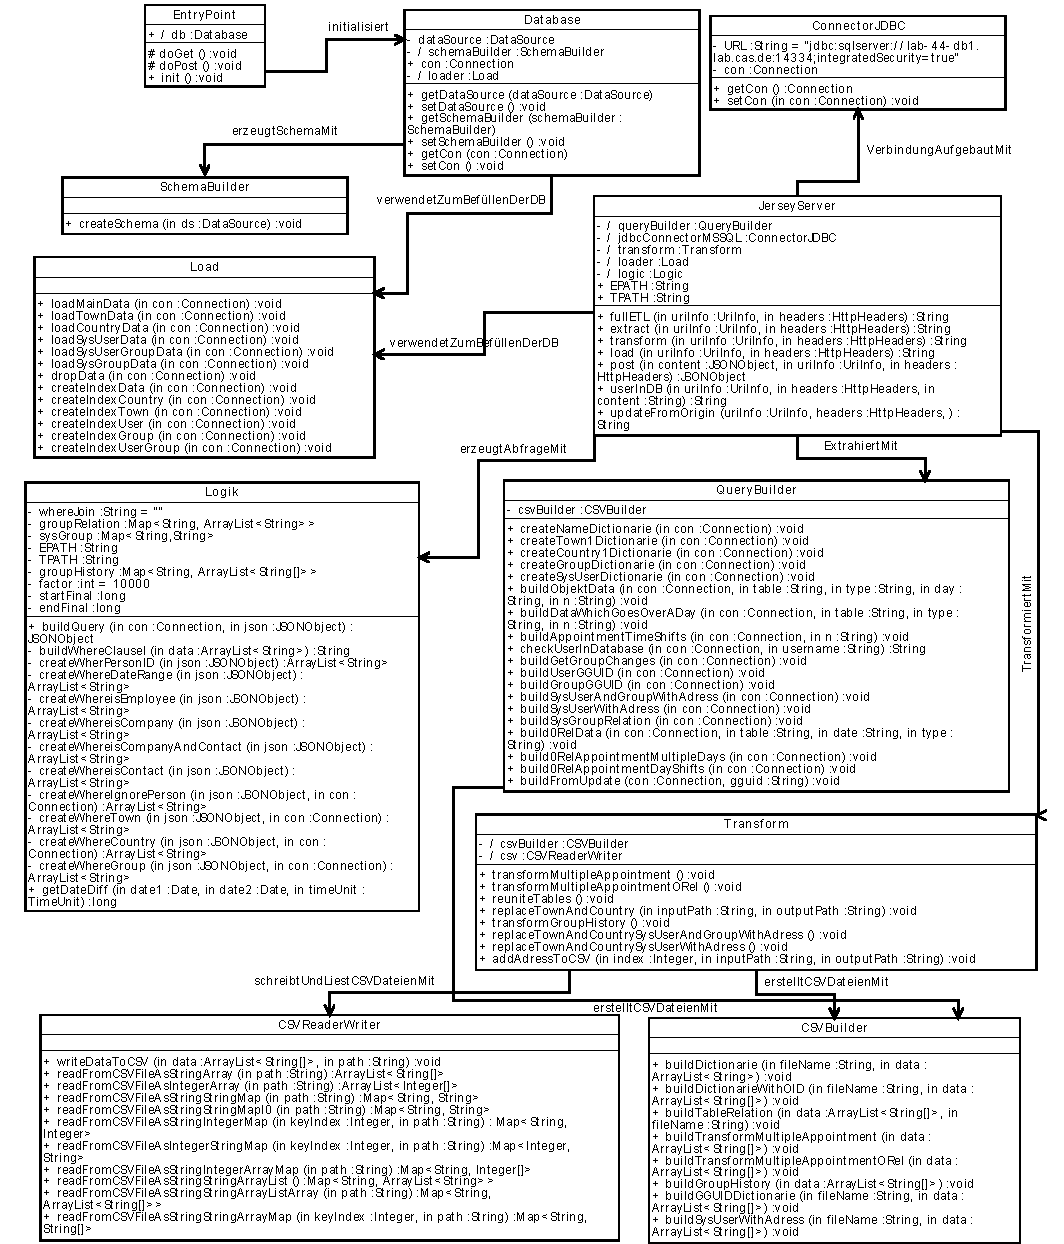
\includegraphics[width=1.0\textwidth]{pics/ServerKlassendiagramm.pdf}
\caption{Server Klassendiagramm}
\label{umsetzung_klassendiagramm_server}
\end{center}
\end{figure}


In den Methoden zur Verarbeitung von REST-Requests werden Methoden die den ETL-Prozess ausführen aufgerufen. Die Klasse  \textit{ConnectorJDBC} besitzt ein Attribut namens \textit{con}, welches den Verbindungsaufbau zum MSSQL-Server, mithilfe von JDBC ermöglicht. Zur Extraktion der Daten aus der MSSQL-Datenbank wird ein Objekt der Klasse \textit{QueryBuilder} verwendet. Wie in der Abbildung zu sehen wird die Extraktion in der Klasse \textit{QueryBuilder} durch mehrere Methoden mit unterschiedlichen Übergabeparametern umgesetzt. Methoden welche die Übergabewerte \textit{table}, \textit{date} und \textit{n} besitzen, werden zum Beschaffen der CRM-Objekte eingesetzt. Mithilfe des Parameters \textit{table} wird der betroffene Tabellenname aus der MSSQL-Datenbank übergeben. Der Parameter \textit{date} gibt das Attribut an, was für die Ermittlung des Datums verwendet werden soll. Um den Typ eines CRM-Objektes zwischen Personen festzuhalten wird der Parameter \textit{n} verwendet, der eine Zahl zwischen eins und fünf beinhaltet. Die unterschiedlichen Bedeutungen sind in der Tabelle \ref{tb:BedeutungDerZahlenQueryBuilder} festgehalten. \textit{QueryBuilder} verwendet ein Objekt der Klasse \textit{CSV-Builder}, um die Ergebnisse der SQL-Abfragen in Dateien festzuhalten. Den Methoden wird als Übergabeparameter ein Dateiname sowie die zu speichernden Informationen übergeben.

\begin{table}[htbp]
\centering
\begin{tabular} {l | r}
Wert & Bedeutung  \\ \hline
1 & E-Mail \\
2 & Dokument \\
3 & Termin \\
4 & Verkaufschance \\
5 & Telefonat \\
\end{tabular}
\caption{Bedeutung der verschiedenen Werte für \textit{n}}
\label{tb:BedeutungDerZahlenQueryBuilder}
\end{table}


Die Klasse \textit{Transform} enthält Attribute und Methoden zur Bearbeitung der in der Extraktion erzeugten CSV-Dateien. Der Inhalt der Dateien wird mithilfe eines \textit{CSVReaderWriter} Objekts ausgelesen und in die Java-Laufzeitumgebung geladen. Nach der Bearbeitung durch die Methoden der \textit{Transform} Klasse, werden die Daten wieder in CSV-Dateien zurückgeschrieben. \textit{CSVBuilder} besitzt Methoden die zusätzliche Parameter zum Schreiben aufweisen, die Anpassungen an den Schreiboperationen erlauben. Wohingegen \textit{CSVReaderWriter} mithilfe der Methode \textit{writeDataToCSV()}, sowie den Parametern \textit{path} und \textit{data} für allgemeine Schreiboperationen verwendet wird.

Mithilfe der Klasse \textit{Load} kann die Datenbank befüllt werden. Sie wird von den \textit{Database} und \textit{JerseyServer} Objekten verwendet. In der Klasse \textit{JerseyServer} wird das Befüllen der Datenbank durch eine Person angestoßen.

In der Klasse \textit{Database} wird die Methode \textit{load()} ebenfalls aufgerufen. Dies findet jedoch einmalig im Konstruktor statt, um die Datenbank beim starten des Anwendungsserver automatisch zu befüllen. Die Klasse \textit{Database} wird dementsprechend lediglich einmal instanziiert. Bei späteren aufrufen wird kein neues Objekt erzeugt sondern eine Referenz des bereits existierenden Objekts übergeben.

Die Klasse \textit{UserQuery} beinhaltet Attribute und Methoden zum Beantworten von Benutzerabfragen. Zur Ermittlung der Bedingungen für die WHERE-Klausel einer SQL-Abfrage werden separate Methoden verwendet. Jede Methode fügt unterschiedliche Bedingungen zur WHERE-Klausel hinzu. Der Aufruf der jeweiligen Methode ist abhängig von der durch den Client übertragenen JSON-Datei. Enthält diese Angaben zum Filtern der Ergebnismenge, so wird die entsprechende Methode aufgerufen. Beispielsweise kann der Nutzer angeben, dass er keine Personen aus Karlsruhe im Ergebnis haben möchte. Diese Angabe wird in Form eines Schlüssel-Werte-Paares im JSON-Format an den Server übermittelt. Der Server ruft bei einem entsprechenden Eintrag im JSON anschließend die Methode \textit{createWhereTown()} auf. Nachdem alle Bedingungen der WHERE-Klausel vorhanden sind, wird die SQL-Abfragen an die H2-Datenbank mithilfe der Methode \textit{buildQuery()} generiert und gesendet. 

%% ===========================
\section{Client-Webprojekt}
\label{ch:Umsetzung:sec:clientwar}
%% ===========================

Der Einstiegspunkt des Webprojekts ist die Klasse \textit{CasAnalyticUI} aus der Abbildung \ref{umsetzung_klassendiagramm_client}. Sie ist von der Vaadin-Klasse \textit{UI} abgeleitet. Die \textit{UI} ist die oberste Komponente jeder Komponentenhierarchie in Vaadin. Es gibt eine Benutzeroberfläche für jede Vaadin-Instanz in einem Browserfenster. Ein \textit{UI}-Objekt kann entweder ein gesamtes Browserfenster (-Tab) oder einen Teil einer HTML-Seite darstellen, in der eine Vaadin-Anwendung eingebettet ist. Nachdem eine \textit{UI} von der Anwendung erstellt wurde, wird diese mit der Methode \textit{init(VaadinRequest)} initialisiert. Zur Übersicht sind die Komponenten der Darstellung in die Klasse \textit{RootUI} ausgelagert. 

Die \textit{RootUI} wird in der \textit{CasAnalayticUI} instanziiert. Die Klasse \textit{RootUI} beinhaltet Objekte die Vaadin-Komponenten zur Darstellung des Anmeldefensters sowie der Hauptansicht. Mithilfe der Methode \textit{buildLoginView()} werden die Komponenten des Anmeldefensters zur \textit{UI}-Komponente hinzugefügt. Nach der Erzeugung der Komponenten, wird eine \textit{JerseyClient} Klasse instanziiert. Diese wird verwendet sobald der Nutzer IP, Port und einen Namen eingegeben hat und sich anmelden möchte. Im Anschluss wird die Methode \textit{doPostRequestUserData()} gerufen, um zu überprüfen ob der Nutzer im System vorhanden ist. 

\begin{figure}[htbp]
\begin{center}
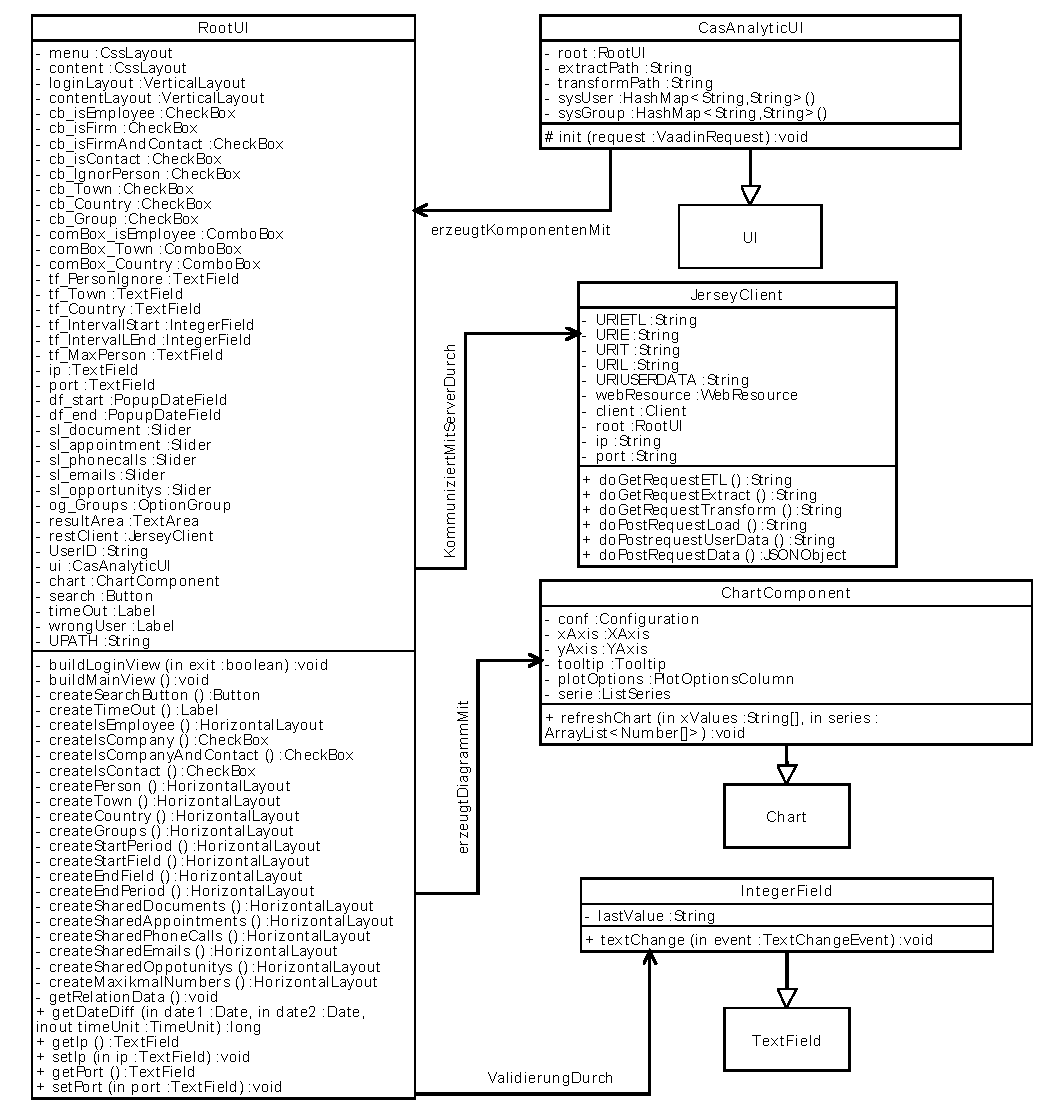
\includegraphics[width=0.9\textwidth]{pics/ClientKlassendiagramm.pdf}
\caption{Client Klassendiagramm}
\label{umsetzung_klassendiagramm_client}
\end{center}
\end{figure}

Falls ja, werden durch die Methode \textit{MainView()} alle Vaadin-Komponenten von der \textit{UI} entfernt und durch neue Vaadin-Komponenten ersetzt. Die neuen Vaadin-Komponenten spiegeln die Hauptansicht der Anwendung wieder. Das \textit{JerseyClient} Objekt wird direkt im Anschluss verwendet, um mithilfe der Methode \textit{doPostRequestData()} einen REST-Request an den Server zu senden. Dieser liefert das Ergebnis der SQL-Abfrage in einem JSON-Objekt zurück, mit dessen eine erste Erzeugung des Diagramms durchgeführt wird. Das Diagramm selbst besitzt eine eigene Klasse namens \textit{ChartComponent}. Sie leitet sich von der Klasse \textit{Chart} ab, die Teil der VaadinChart-Bibliothek ist. Mithilfe der Methode \textit{refreshChart()} wird das Diagramm bei Benutzerabfragen aktualisiert. Dazu werden ihr die Namen der Personen für die x-Achse übergeben sowie die Wertigkeiten der Beziehungen für die y-Achse. Weiterhin wird für jede Vaadin-Komponente eine separate Methode zur Konfiguration verwendet. Änderungen am Aussehen oder an der Funktionalität der jeweiligen Vaadin-Komponenten, werden nur innerhalb der entsprechenden Methode vorgenommen.

An der Oberfläche gibt es Eingabefelder die nur Zahlen erwarten. Eingaben die nicht numerisch sind werden durch den Einsatz der Klasse \textit{IntegerField} verhindert. Diese erweitert die Klasse \textit{TextField}. Sie besitzt einen Event-Listener, der jede Eingabe des Benutzers abfängt. Gibt der Nutzer nicht numerische Zeichen ein werden diese direkt wieder entfernt. Dadurch werden Falscheingaben durch den Nutzer ausgeschlossen.

%% ===========================
\section{Aufbau der H2-Datenbankabfrage}
%% ===========================

Die Abfrage an die H2-Datenbank ist geschachtelt aufgebaut und unterteilt sich in eine innere und äußere Abfrage. In Abbildung \ref{umsetzung_sql} sind die Ergebnisse der inneren und äußeren Abfrage abgebildet. Die Tabelle (A) zeigt einen aufs wesentliche reduzierten Ausschnitt der Datenbasis. Im Beispiel aus der Abbildung \ref{umsetzung_sql} wird die Person mit der \textit{startID} 1 zur Bewertung von Beziehungen ausgewählt. Mithilfe der ersten Abfrage wird zuerst die Anzahl der jeweiligen CRM-Objekte zwischen der Person mit der 1 als ID und allen anderen Personen ermittelt. Die \textit{endID} gibt die jeweilige Person an mit der CRM-Objekte geteilt werden. Das Ergebnis ist in der Tabelle (B) zu sehen. In ihr ist beispielsweise zu erkennen, dass die betrachtete Person 8 Dokumente mit einer Person teilt, welche die \textit{endID} 3 besitzt. Die Tabelle (B) enthält allerdings noch nicht alle benötigten Informationen. Um an diese zu gelangen wird basierend auf der Tabelle (B) die zweite Abfrage gestellt. Dessen Ergebnis ist in der Tabelle (C) dargestellt. In ihr ist die Anzahl der verschiedenen CRM-Objekte in einer Tupel festgehalten. Weiterhin enthält sie die Summe aller CRM-Objekte zu den jeweiligen Personen. Diese wird verwendet um eine absteigende Reihenfolge zu bilden. Diese Reihenfolge bildet eine Ranking unter den Beziehungen der Person. In der Implementierung werden die beiden Abfragen als eine geschachtelte SQL-Abfrage formuliert.

Mit der bisherigen Abfrage kann der Wert einer Beziehung ermittelt werden, allerdings werden mit diesem Vorgehen noch nicht alle Funktionen abgedeckt, sie stellt allerdings die Basisfunktonalität dar. Diese kann durch Eingaben der Nutzer erweitert werden. Diese zusätzlichen Parameter die vom Benutzer übergeben werden, müssen in der SQL-Abfrage berücksichtigt werden. Um die SQL-Abfrage so schlank wie möglich zu halten werden die optionalen Konfigurationen nur bei Bedarf in die SQL-Abfrage aufgenommen. Ein Beispiel dafür ist die Gewichtung von Zeit, die eine höhere Komplexität der Abfrage bewirkt und nur bei einer entsprechenden Angabe durch den Benutzer in die SQL-Anweisung einfügt wird.

\begin{figure}[htbp]
\centering
  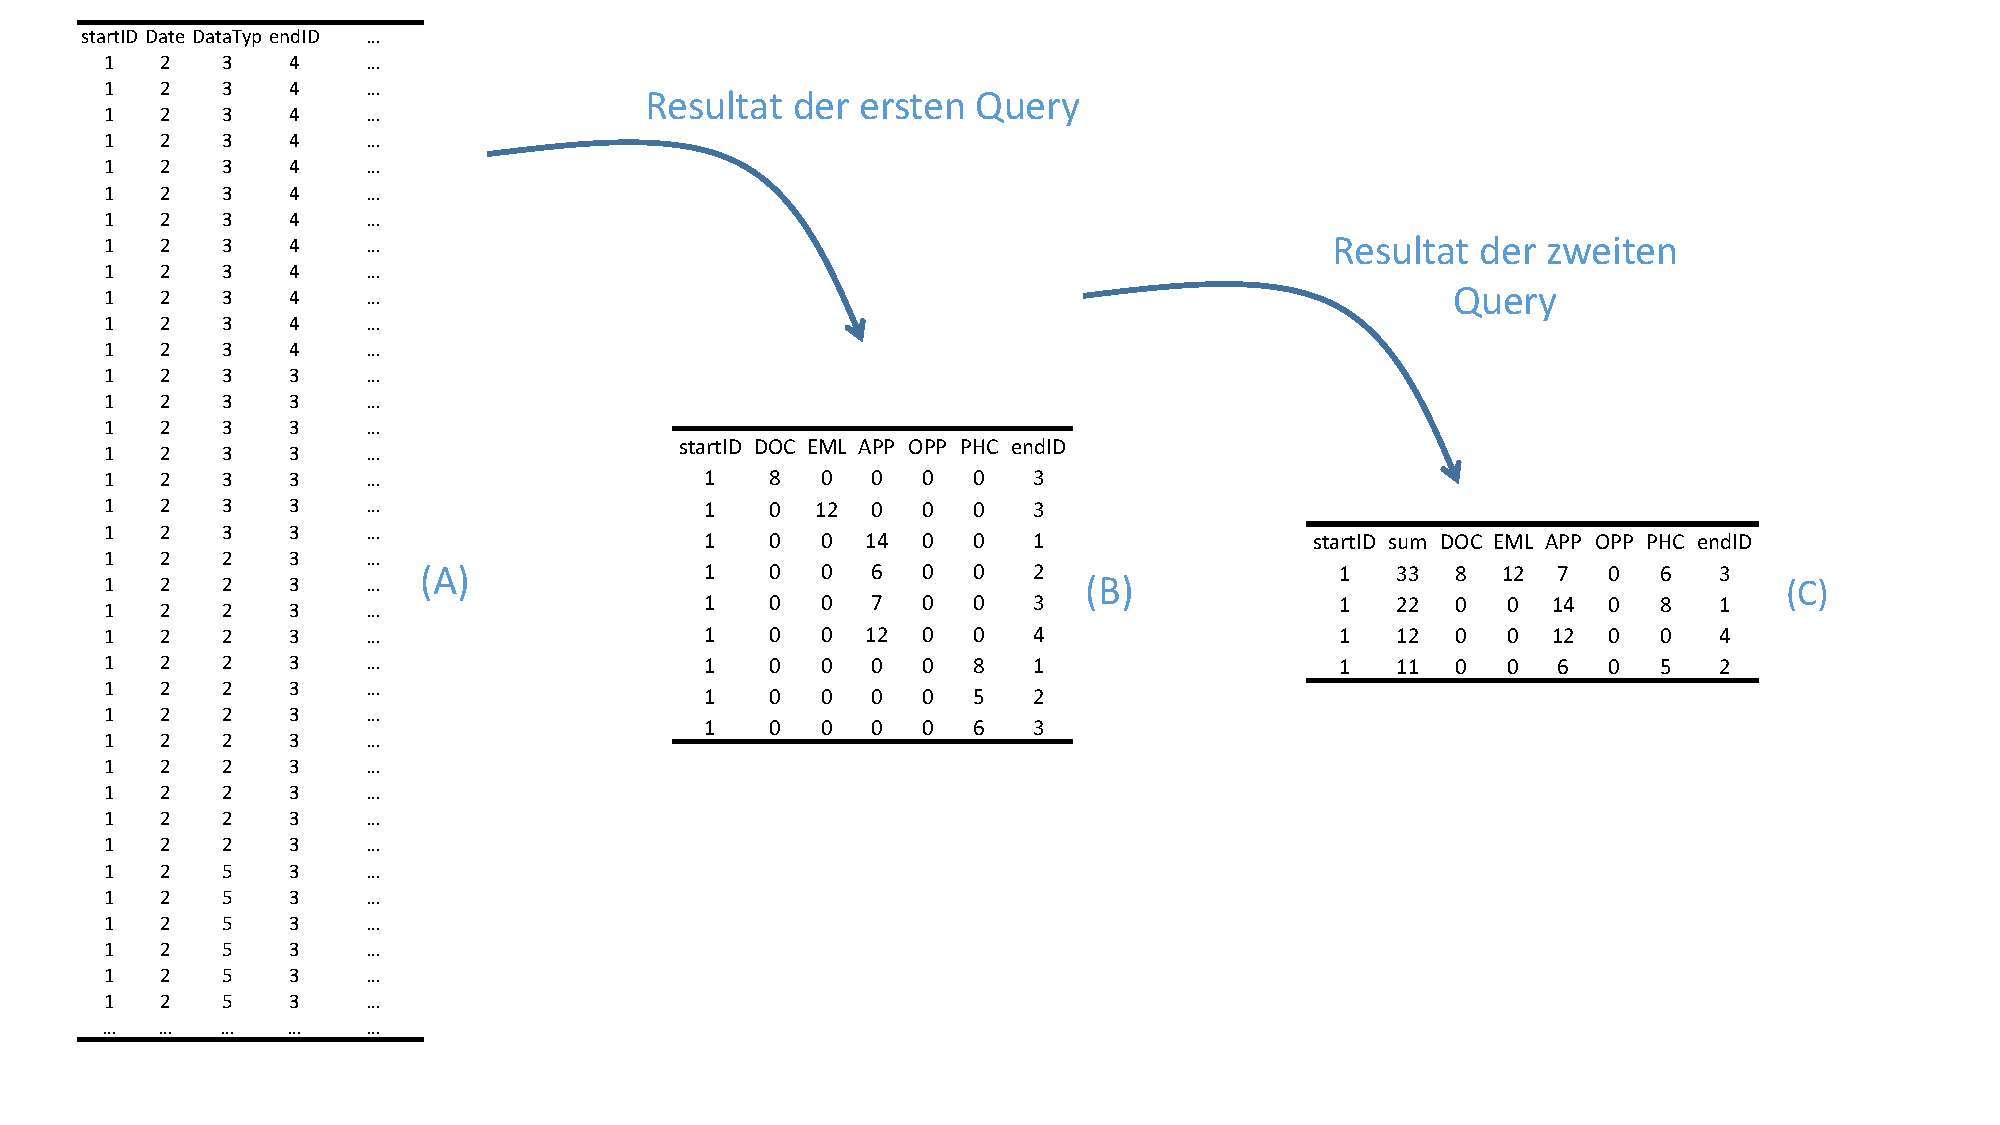
\includegraphics[width=1.0\textwidth]{pics/sql_abfrage.pdf}
\caption{Ergebnisse der verschachtelten SQL-Abfrage}
\label{umsetzung_sql}
\end{figure}

Das Verfahren zur Gewichtung der Zeit wird anhand der Abbildung \ref{fig:umsetzung:gewichtungderzeit} erläutert. Die Abbildung zeigt ein Koordinatensystem mit der Gewichtung von einzelnen Zeitpunkten. Die x-Achse stellt den zeitlichen Verlauf und die y-Achse die Gewichtung dar. Der Startzeitpunkt wird durch $t_{s}$ markiert, wohingegen $t_{e}$ den Endzeitpunkt angibt. Mithilfe von $t_1$ und $t_2$ werden die Zeitpunkte angegeben bis zu denen differenziert gewichtet werden soll. Um nun die Zeitspannen zwischen $t_{s}$-$t_1$ und $t_2$-$t_{e}$ anders zu gewichten wird jedem Tag eine andere Wertigkeit zugewiesen. Dabei werden die Tage linear steigend oder fallend bewertet. Für die Zeitspanne zwischen $t_{s}$ und $t_1$ bedeutet dies, dass der Wert eines Tages zunehmend steigt. Wird $t_1$ erreicht, besitzt jeder Tage wieder eine Wertigkeit von 1. Bei $t_2$ verhält es sich ähnlich. Mit jedem Tag ab $t_2$ sinkt der Wert des Tages bis der Zeitpunkt $t_{e}$ erreicht ist. Der Wert eines Tages wird mit einer Zahl ($\le1$) gekennzeichnet. Außerdem werden alle vier Zeitpunkte durch den Nutzer festgelegt.  

\begin{figure}[htbp]
\begin{center}
\begin{tikzpicture}[domain=-1:2] \draw[very thin,color=gray] (0,0); 
\draw[->] (0,0) -- (12.3,0) node[right] {Zeit}; 
\draw[->] (0,0) -- (0,4.2) node[above] {Gewichtung}; 
\draw[color=black]  (0.2,3) -- (-0.2,3)   node[left] {100\%};
\draw[color=black]  (0.2,1.5) -- (-0.2,1.5)   node[left] {50\%};  
%\draw[dashed][color=black]  (4,0.5) -- (4,3.5); 
%\draw[dashed][color=black]  (9,0.5) -- (9,3.5);

\draw[color=black]  (0,0) -- (0,0)   node[below] {$t_{s}$}; 
\draw[color=black]  (4,0.1) -- (4,-0.1)   node[below] {$t_1$}; 
\draw[color=black]  (9,0.1) -- (9,-0.1)   node[below] {$t_2$};
\draw[color=black]  (12,0.1) -- (12,-0.1)   node[below] {$t_{e}$};   
 
\draw[color=black]  (0,0) -- (4,3)   node[right] {}; 
\draw[color=black]  (4,3) -- (9,3)   node[right] {}; 
\draw[color=black]  (9,3) -- (12,0)   node[right] {};  

\draw[dotted][color=black]  (1,0.75) -- (2,0.75);
\draw[dotted][color=black]  (2,1.5) -- (3,1.5);
\draw[dotted][color=black]  (3,2.25) -- (4,2.25);
\draw[dotted][color=black]  (4,3) -- (5,3);

\draw[dotted][color=black]  (1,0.75) -- (1,0);
\draw[dotted][color=black]  (2,1.5) -- (2,0);
\draw[dotted][color=black]  (3,2.25) -- (3,0);
\draw[dotted][color=black]  (4,3) -- (4,0);
\draw[dotted][color=black]  (5,3) -- (5,0);
\draw[dotted][color=black]  (6,3) -- (6,0);
\draw[dotted][color=black]  (7,3) -- (7,0);

\draw[dotted][color=black]  (8,3) -- (8,0);
\draw[dotted][color=black]  (9,3) -- (9,0);
\draw[dotted][color=black]  (10,2) -- (10,0);
\draw[dotted][color=black]  (11,1) -- (11,0);

\draw[dotted][color=black]  (8,3) -- (9,3);
\draw[dotted][color=black]  (9,2) -- (10,2);
\draw[dotted][color=black]  (10,1) -- (11,1);

\draw[dashed][color=black]  (1,0.75) -- (1,1.05)   node[above] {$t_{s}+1$}; 
\draw[dashed][color=black]  (2,1.5) -- (2,1.8)   node[above] {$t_{s}+2$}; 
\draw[dashed][color=black]  (3,2.25) -- (3,2.55)   node[above] {$t_{s}+3$};  

\draw[dashed][color=black]  (10,2) -- (10,2.3)   node[above] {$t_{e}-2$}; 
\draw[dashed][color=black]  (11,1) -- (11,1.3)   node[above] {$t_{e}-1$}; 

\end{tikzpicture} 
\end{center}
\caption{Gewichtung der Zeit}
\label{fig:umsetzung:gewichtungderzeit}
\end{figure}

Um eine lineare Gewichtung der Tage zu erzielen werden zuerst die Steigungen zwischen den Zeitpunkten berechnet:

\begin{equation}
s_1 = \frac{1}{t_1 - t_{s}}
\end{equation}
\begin{equation}
s_2 = \frac{1}{t_{e} - t_2}
\end{equation}

Mit den Steigungen können nun die Werte der Tage berechnet werden. Das Vorgehen dafür wird im Folgenden anhand der Zeitspanne zwischen $t_{s}$ und $t_1$ erläutert. Bei jeder betrachteten Tupel in der Datenbankabfrage wird überprüft, ob sie sich in der angegebenen Zeitspanne befindet. Ist dies der Fall wird zuerst die Differenz zwischen dem Datum der aktuellen Tupel und dem Zeitpunkt $t_{s}$ ermittelt. Die Differenz wird anschließend mit der Steigung multipliziert, wodurch sich die Wertigkeit des jeweiligen Tages ergibt. Der Zeitpunkt $t_{s}$ weist somit immer einen Wert von 0 auf, wohingegen $t_1$ immer den Wert 1 besitzt. Zwischen den beiden steigt der Wert eines Tages stufenweise an. 

Die Auswirkungen dieser zusätzlichen Abläufe sind in der Abbildung \ref{umsetzung_sql2} dargestellt. Es zeigt mit Beispielwerten wie die Tabelle (A) aus der Abbildung \ref{umsetzung_sql} um eine weitere Spalte ergänzt wird, welche die berechneten Werte enthält. Das darauf folgende Vorgehen unterscheidet sich von der in Abbildung \ref{umsetzung_sql} gezeigten nur in einem Punkt. Das Resultat der ersten Query zählt nicht mehr einfach die Häufigkeit der CRM-Objekte zu einer Person, sondern bildet Summen aus den entsprechenden Werten der Spalte \textit{TagGew}. Dieser werden anschließend in den Spalten der CRM-Objekte in der Tabelle (B) aus der Abbildung \ref{umsetzung_sql2} vermerkt.  

\begin{figure}[htbp]
\centering
  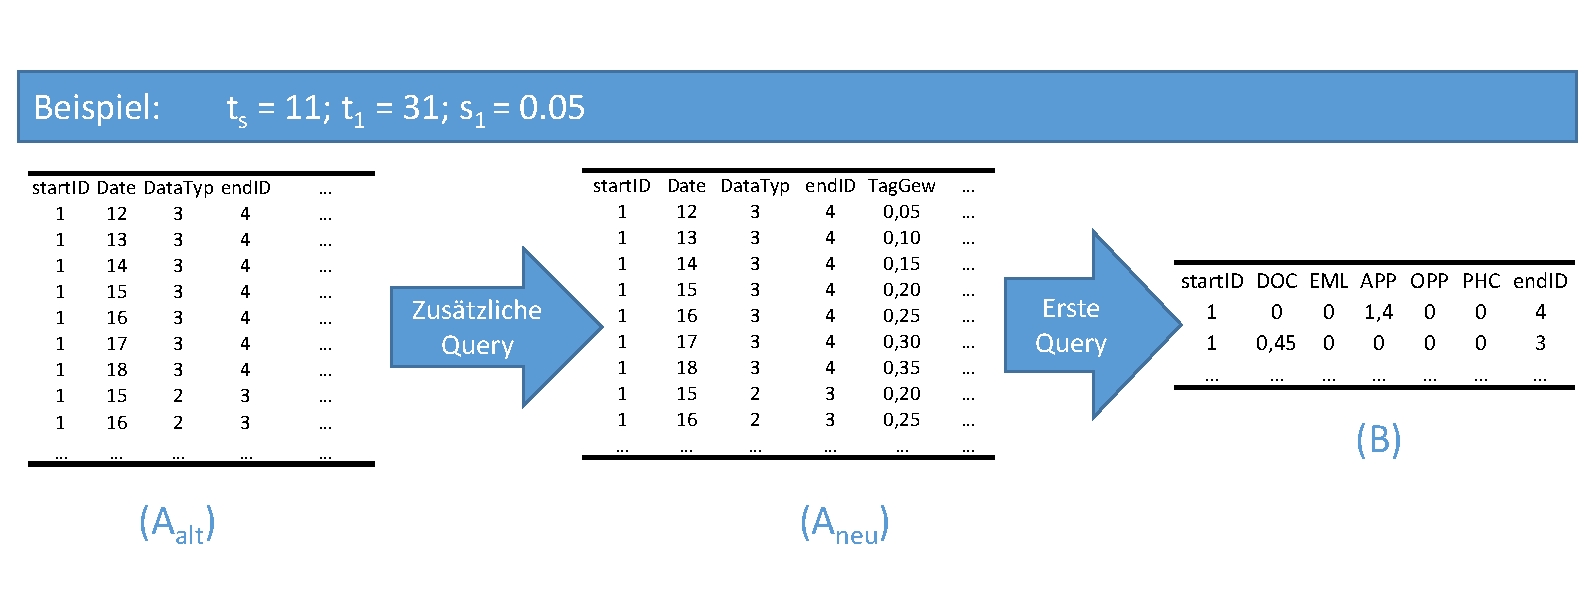
\includegraphics[width=1.0\textwidth]{pics/sql_abfrage2.pdf}
\caption{Beispiel der zusätzlichen SQL-Abfrage zur Gewichtung der Zeit}
\label{umsetzung_sql2}
\end{figure}

Zur Umsetzung des zuvor beschriebenen wird die SQL-Anweisung um eine weitere Abfrage erweitert. Diese Abfrage wird zuerst gestellt, da nach den anderen Abfragen kein Datum mehr vorhanden ist. 

Neben der Zeit lassen sich die jeweiligen CRM-Objekte unterschiedlich gewichten. Dazu wird lediglich die Summe des jeweiligen CRM-Objekttyps um einen angegebenen Prozentsatz reduziert. Diese Gewichtung findet in der ersten Abfrage statt. 

%Es handelt sich dabei um Gruppen, dessen Personen aus der Ergebnismenge auszuschließen sind. Ihre Konstellation in Bezug auf Personen ist im Laufe der Zeit variabel. Um dies zu berücksichtigen wird die Tabelle \textit{UserGroup} verwendet. Dabei wird folgendermaßen vorgegangen: 

%Zuerst wird für jede Gruppe ein eigenes Array in der Java-Laufzeitumgebung erzeugt. Das Array beinhaltet die IDs der Personen aus der jeweiligen Gruppe. Liegt nun der Zeitpunkt des Feldes \textit{Date} nach dem Anfangszeitpunkt der Abfrage und die Spalte \textit{Action} enthält eine 1, wird das Array um diese Person reduziert. Enthält sie eine 0, wird die Person zum Array hinzugefügt. Mit einer 1 in der Spalte \textit{Action} wird der Austritt einer Person aus der Gruppe markiert. Eine 0 weist auf den Eintritt einer Person in die Gruppe hin. Dadurch wird die Struktur der Gruppe zum Anfangszeitpunkt wiederhergestellt. Mithilfe des Array werden anschließend die WHERE-Klauseln um weitere auszuschließende Personen erweitert.

%Innerhalb von Zeiträumen können sich Gruppen auch verändern, jedoch kann dies nicht berücksichtigt werden. Es kann jeweils nur ein bestimmter Zeitpunkt betrachtet werden. In diesem Fall wurde der Anfangszeitpunkt $t_{s}$ ausgewählt.

%% ===========================
\section{ETL-Prozess}
%% ===========================

Die Vorgehensweise der Extraktion wird anhand der Abbildung \ref{umsetzung_extract} erläutert. Jeder Pfeil stellt einen Verbund zwischen den jeweiligen Tabellen dar. Das Vorgehen in der Abbildung zeigt wie die Datensätze für die Tabelle \textit{Data} ermittelt werden. 

\begin{figure}[htbp]
\centering
  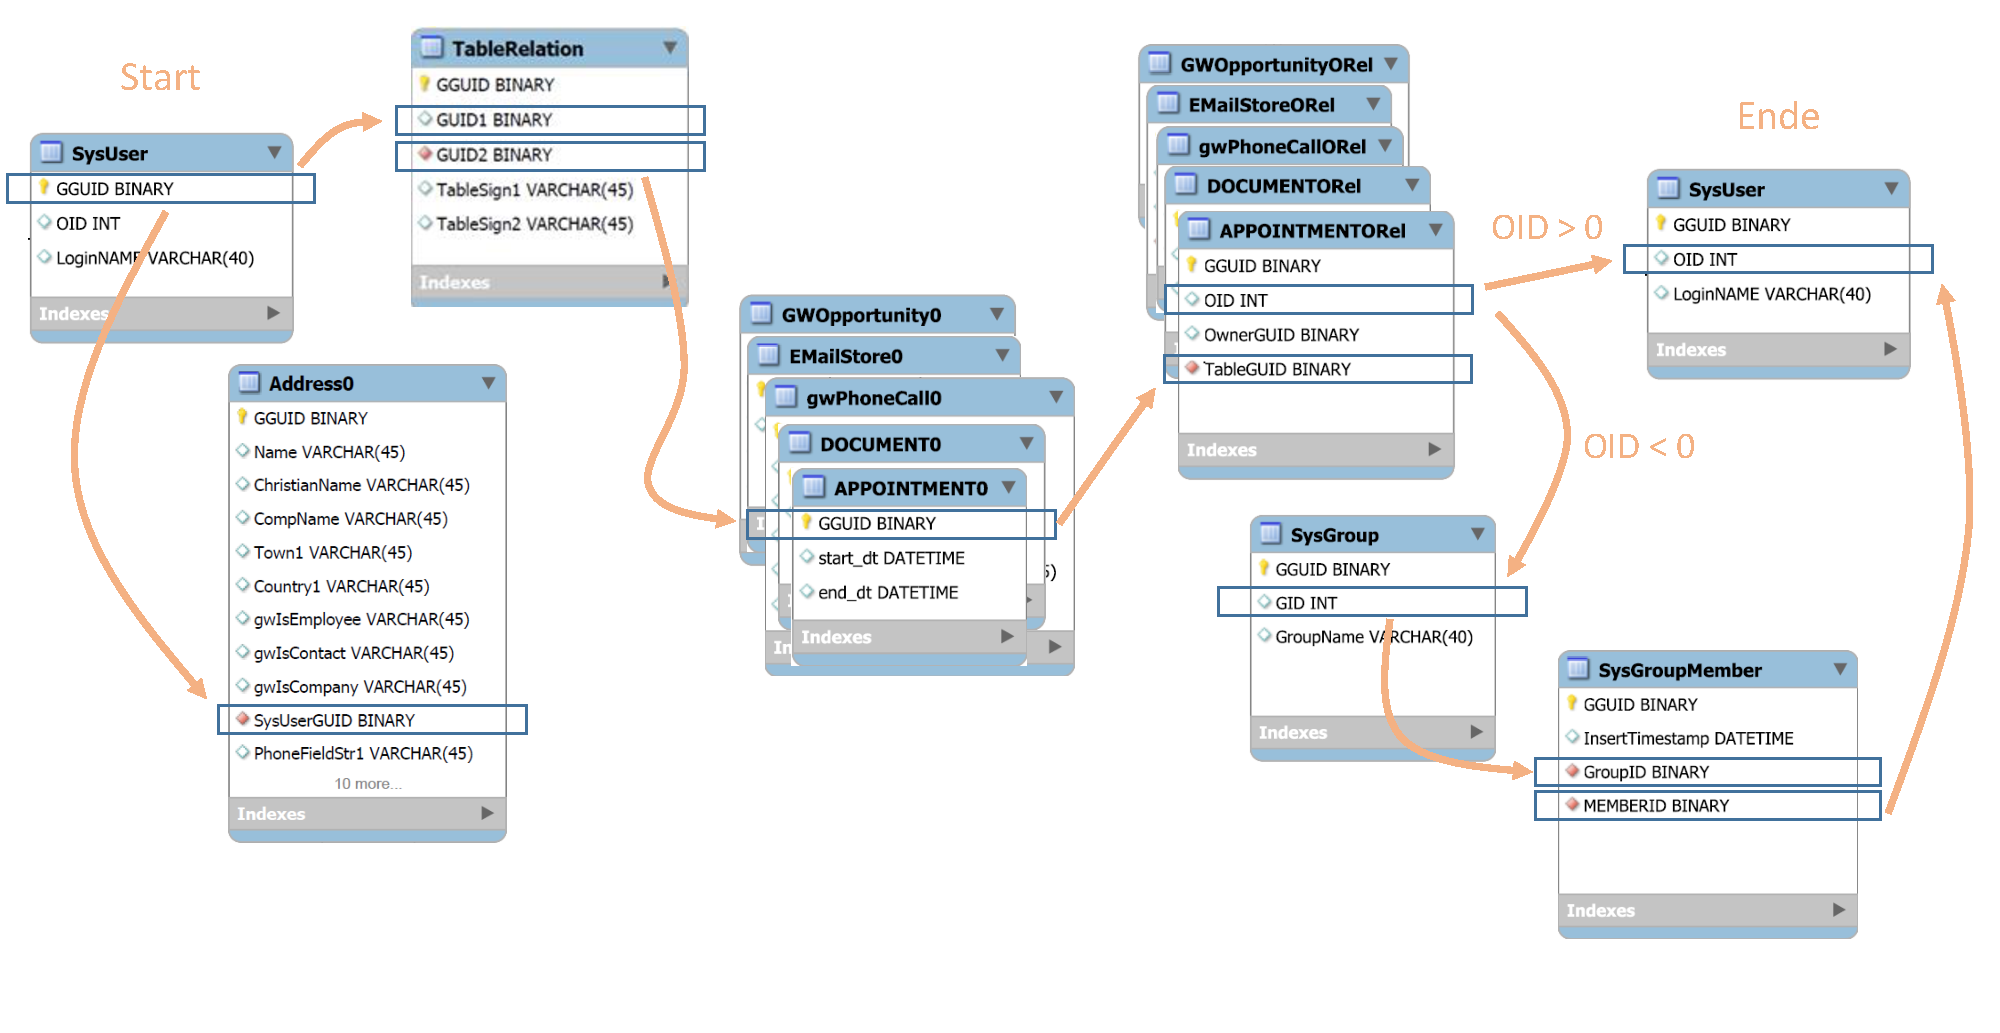
\includegraphics[width=1.0\textwidth]{pics/konzept_extraktion.pdf}
\caption{Vorgehensweise bei der Extraktion}
\label{umsetzung_extract}
\end{figure} 

Die erste Information entstammt der Tabelle \textit{SysUser}. Mithilfe eines Verbundes zwischen den Tabellen \textit{SysUser} und \textit{Address0} werden die persönlichen Daten zu den Personen ermittelt. Anschließend werden durch einen Verbund zwischen \textit{TableRelation} und \textit{SysUser} alle Tabellen bestimmt, mit denen die Personen eine Verknüpfung besitzen. Der nächste Verbund wird zwischen \textit{TableRelation} und den Tabellen \textit{gwOpportunity}, \textit{gwPhoneCall0}, \textit{Document0}, \textit{EmailStore0} und \textit{Appointment0} gebildet. Dadurch werden alle CRM-Objekte der Personen ausgemacht. Um beispielsweise festzustellen mit welchen anderen Personen ein Dokument geteilt ist, wird ein weiterer Verbund mit der passenden \textit{ORelDocument0}-Tabelle gebildet. In der ORel-Tabelle kann der Wert der \textit{OID} positiv, sowie negativ sein. Bei einem negativen Wert stellt die \textit{OID}, eine \textit{GID} der Tabelle \textit{SysGroup} dar. Ist der \textit{OID}-Wert in der ORel-Tabelle positiv, weist dies auf einen Fremdschlüssel der Tabelle \textit{SysUser} hin. Bei den anderen CRM-Objekten verhält es sich genauso wie bei dem Beispiel mit dem Dokument.

Zur Auflösung von Gruppen in einzelne Personen werden folgende Verbunde gebildet. Zuerst zwischen \textit{SysGroup} und \textit{SysGroupMember}, um alle Personen die zu einer Gruppe gehören zu erhalten. Anschließend zwischen \textit{SysGroupMember} und \textit{SysUser}, um die \textit{OID} der Person zu bestimmen.

Die durch den Verbund gewonnen Informationen werden innerhalb der SQL-Anweisung auf die 9 relevanten Attribute der \textit{Data}-Tabelle reduziert. Zu einem die \textit{OID} des \textit{SysUser}, von dem die Suche ausgeht. Zum anderen das Datum, welches durch das CRM-Objekt ermittelt wird. Weiterhin wird die zweite \textit{OID} beibehalten, die durch den Verbund mit einer zweiten \textit{SysUser} Tabelle gewonnen wird. Zum Schluss wird eine vierte Information hinzugefügt, die besagt welcher CRM-Objekttyp  zwischen den beiden Personen geteilt wird. Weiterhin werden die restlichen fünf Werte der \textit{Data}-Tabelle aus der \textit{Adress0} übernommen. 

Für den Sonderfall, dass ein Datum über mehrere Tage geht, wird ein zehnter Wert an das Ergebnis angehängt, welche den Zeitraum in Tagen beinhaltet. Zur Beschaffung der geschobenen Termine wird die gleiche Abfrage wie zuvor gestellt, allerdings mit einem Verbund zwischen der Tabelle Appointment0 und \textit{ChangeLogBook}. Dadurch kann zum bestimmen der betroffenen Termine wie in Kapitel \ref{ch:konzeption:etl:extract} beschrieben vorgegangen werden.

Jedes Ergebnis einer Datenbankabfrage wird in einer CSV-Datei auf dem Tomcat-Server gespeichert. Diese CSV-Dateien stellen die Grundlage der Transformation dar. Jede dieser Dateien beinhaltet Werte für die Tabelle \textit{Data} aus der H2-Datenbank, in der Form wie sie in Abbildung \ref{fig:umsetzung_csv_datei} zu sehen ist. 

Alle CSV-Dateien werden auf die in Abbildung \ref{fig:umsetzung_csv_datei} zu sehenden Anomalien untersucht. Bei Nullwerten wird überprüft ob wirklich keine Adresse vorhanden ist, falls doch wird die Adresse ergänzt. In Zeile 41 ist zu sehen, dass ein Nullwert anstatt eines Datums vorkommen kann. Diese Zeilen werden aus den CSV-Dateien entfernt. Wenn wie in Zeile 42 ein zusätzlicher Wert am Ende der Zeile vorhanden ist, erstreckt sich die Dauer des CRM-Objektes über die angegebene Anzahl von Tagen. In der Zeile 42 aus dem Beispiel sind es drei Tage. Die Zeile bleibt nach der Transformation bestehen, allerdings wird der letzte Wert entfernt. Die Zahl wird jedoch zwischengespeichert und zur Erzeugung der entsprechenden Anzahl von Tupeln wiederverwendet. Bei einer Dauer von drei Tagen würde die Zahl entfernt und zwei weitere Tupeln in die Datei eingefügt werden. Jede Tupel würde einen anderen Tag in der Zeitspanne des CRM-Objektes darstellen. Nach der Beseitigung von Anomalien werden noch die Städte und Länder durch ihre jeweilige \textit{ID} aus der Tabelle \textit{Town} und \textit{Country} ersetzt.

\begin{figure}[htbp]
\begin{center}
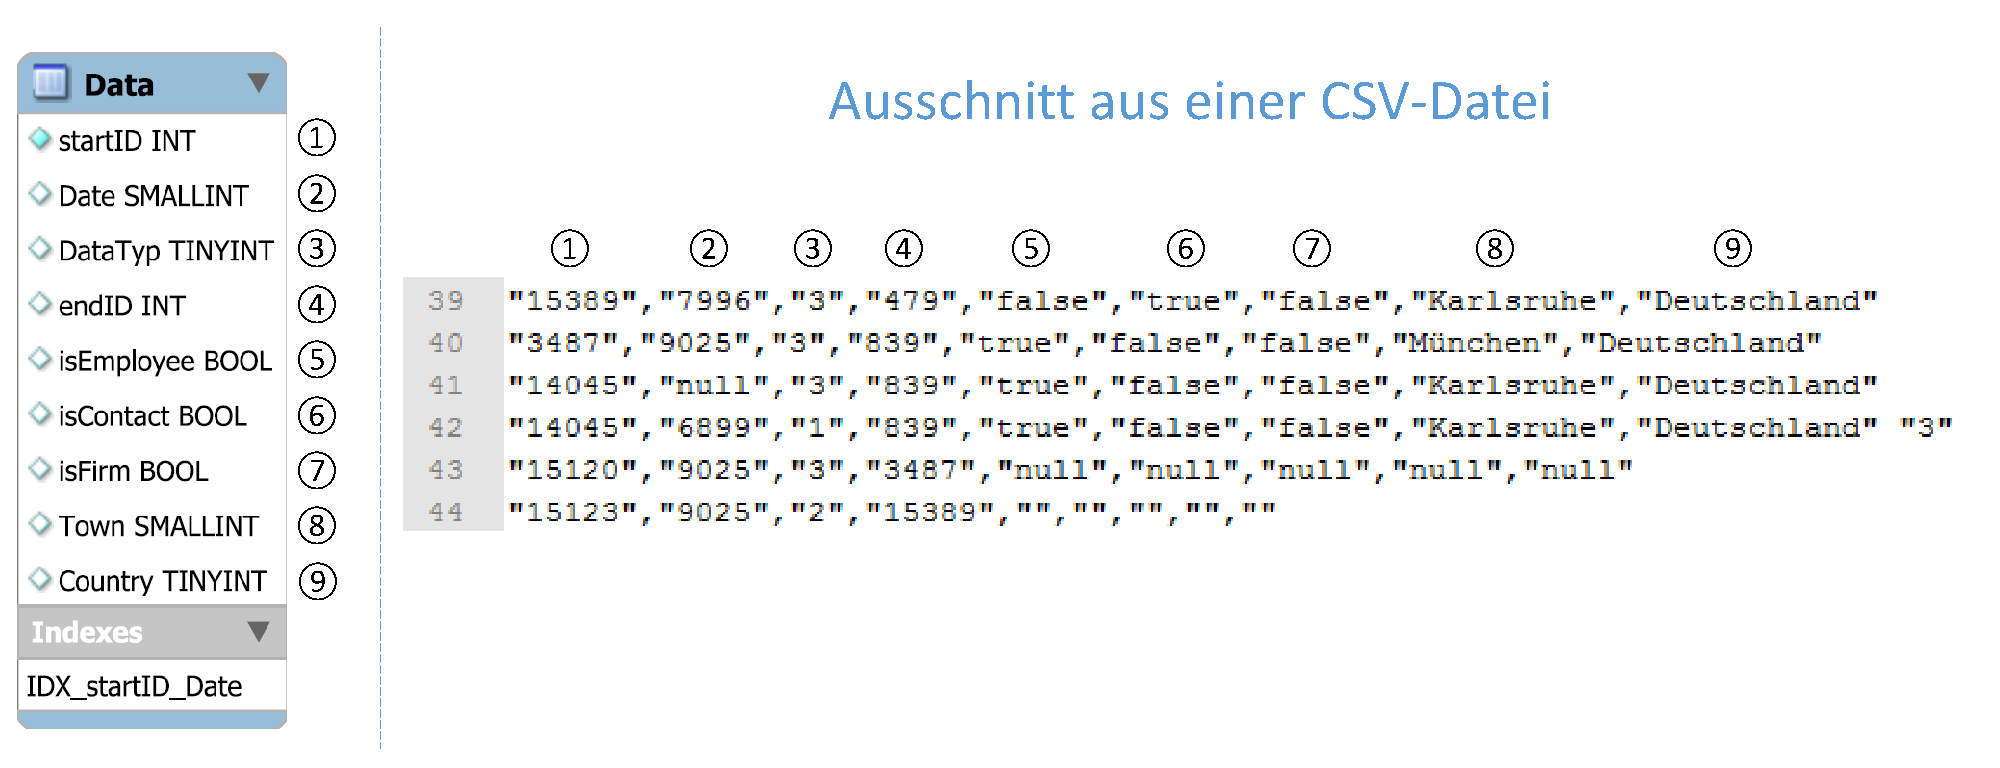
\includegraphics[width=1.0\textwidth]{pics/umsetzung_transformation.pdf}
\caption{Ausschnitt einer CSV-Datei nach der Extraktion}
\label{fig:umsetzung_csv_datei}
\end{center}
\end{figure}

Die überprüften Daten werden wieder in CSV-Dateien abgelegt. Diese besitzen den gleichen Namen, allerdings wird noch der Zusatz "\_transf" angehängt, der sie als transformiert kennzeichnet. Diese Dateien werden anschließend in der Java-Laufzeitumgebung zusammengeführt. Bei der Zusammenführung sind zum ersten Mal alle Daten gleichzeitig in der Anwendung vorhanden und werden für das spätere einspielen sortiert. Dabei wird mit zwei Kriterien verfahren. Das erste Kriterium ist die \textit{OID} (erster Wert in einer Zeile) der Person von der die Suche ausgeht. Als weiteres Sortierkriterium wird das Datum (zweiter Wert in einer Zeile) verwendet. Nachdem alle Zeilen sortiert sind, werden sie in einer CSV-Datei abgelegt. 

Diese Datei wird bei jedem Start der Datenbank verwendet, um einen Bulk-Load für die H2-Datenbank zu initialisieren. Dies ist notwendig, da im In-Memory-Modus die Daten der H2-Datenbank nicht persistent sind und sie nach jedem beenden der Datenbank gelöscht werden. Nachdem Einspielen der Daten in die Datenbank, werden anschließend die Indizes der Datensätzen erzeugt.

%% ===========================
\section{Aktualisierung des Datenbestandes}
%% ===========================

Wie zuvor in Abschnitt \ref{ch:Konzeption:architektur} behandelt, wird die Aktualisierung unseres Datenbestandes von CAS genesisWorld angestoßen. Die Implementierung ist in Form einer COM-Komponente umgesetzt. Sie wird in einer DLL-Datei definiert. Diese muss Namenskonventionen einhalten. Es werden nur Dateien vom CAS genesisWorld Anwendungsserver erkannt die mit dem Prefix \textit{pGSAxExtCustomServerDataPlugin} beginnen. Der Name der DLL-Datei ist in der \textit{RegisterSDKDataPlugIns.xml} hinterlegt, damit der Anwendungsserver beim Start das Plugin findet. Weiterhin ist in der XML-Datei eine Tabelle immer paarweise mit einer DLL angegeben. Dadurch wird ein Plugin auf eine Datenbanktabelle registriert und bekommt alle betreffenden Änderungen mit.

Die Programmbibliothek selbst ist in Delphi geschrieben. Abbildung \ref{ergebniss_plugin_klassendiagramm} zeigt die Struktur der DLL-Datei. Die Klasse selbst implementiert sechs verschiedene Schnittstellen. \textit{ComObj} stellt Funktionen zur Erstellung und Bearbeitung von COM-Objekten zur Verfügung. Um Funktionalitäten von CAS genesisWorld vollständig zu nutzen, wird die \textit{ActiveX} Schnittstelle benötigt. Wie bereits behandelt findet die Übertragung der Daten über das REST-Protokoll statt, wofür die Methoden der \textit{idHttp}\footnote{idHttp ist eine Delphi-Schnittstelle die eine Implementierungen der HTTP-Befehle darstellt (z.B. GET oder POST)} Schnittstelle verwendet werden. Um Konvertierungen der vom Anwendungsserver erhaltenen Binärwerte vorzunehmen, werden die Funktionen der Schnittstellen \textit{CAS\_ToolsCOM} und \textit{CAS\_VarType14Fix} genutzt. Das Abfangen der geänderten Daten, welches die eigentliche Kernfunktionalität darstellt, wird durch die Funktionen der \textit{IGWSDKDataPlugin} Schnittstelle implementiert.

\begin{figure}[htbp]
\centering
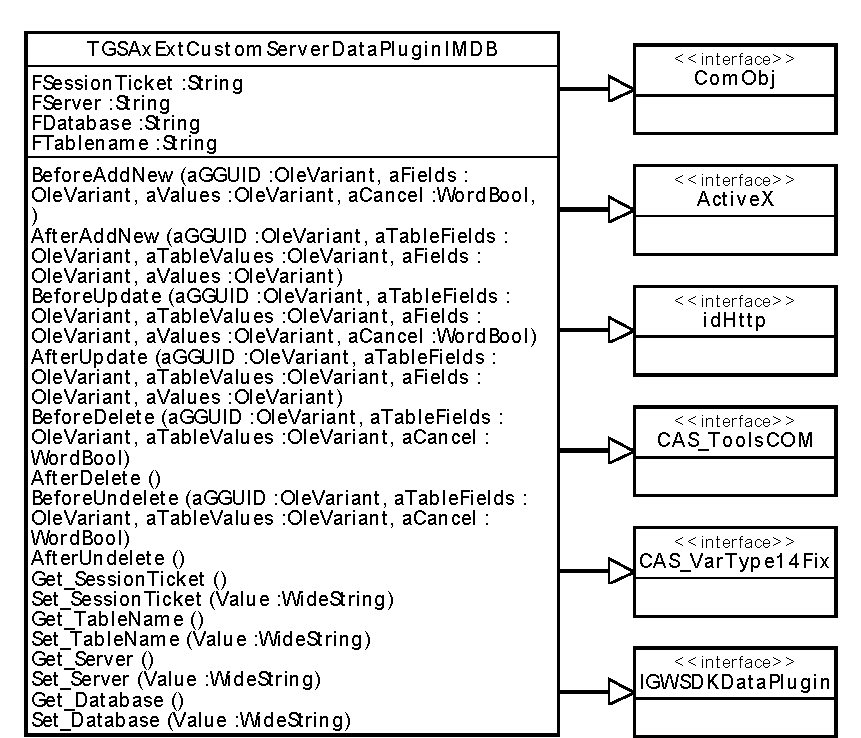
\includegraphics[scale=0.7]{pics/plugin_klassendiagramm.pdf}
\caption{Klassendiagramm Plugin}
\label{ergebniss_plugin_klassendiagramm}
\end{figure}

Die Funktionen \textit{BeforeAddNew()} bis \textit{AfterUndelete()} aus der Abbildung \ref{ergebniss_plugin_klassendiagramm} gehören zu genau di \textit{IGWSDKDataPlugin} Schnittstelle. Es sind zwar alle Funktionen der Schnittstelle in der DLL-Datei implementiert, allerdings sind nur die mit \textit{"After"} beginnen auch mit Logik hinterlegt. Für unser System reicht es aus, über Änderungen im Nachhinein benachrichtigt zu werden. Die Funktionen enthalten alle die gleiche Logik und unterscheiden sich lediglich in den Übergabeparameter.

Die Funktionsweise wird im Folgenden anhand der Kommunikationen beim Anlegen eines neuen Datensatzes durch einen CAS genesisWorld Client erläutert und in der Abbildung \ref{umsetzung_sequenz} dargestellt. Nachdem ein Benutzer einen neuen Datensatz angelegt hat wird das Plugin benachrichtigt. Die Funktion \textit{BeforeAddNew()} enthält die \textit{GGUID} der Tupel, den Namen der Spalte, sowie die neuen Werte des Datensatzes. In unserem Plugin führt das zu keiner Reaktion an dieser Stelle, da wir erst auf Änderungen im Nachhinein reagieren. Im Anschluss an die Benachrichtigung wird der neue Datensatz in die MSSQL-Datenbank eingefügt. Nachdem das passiert ist werden die registrierten Plugins wieder benachrichtigt.

\begin{figure}[htbp]
\centering
  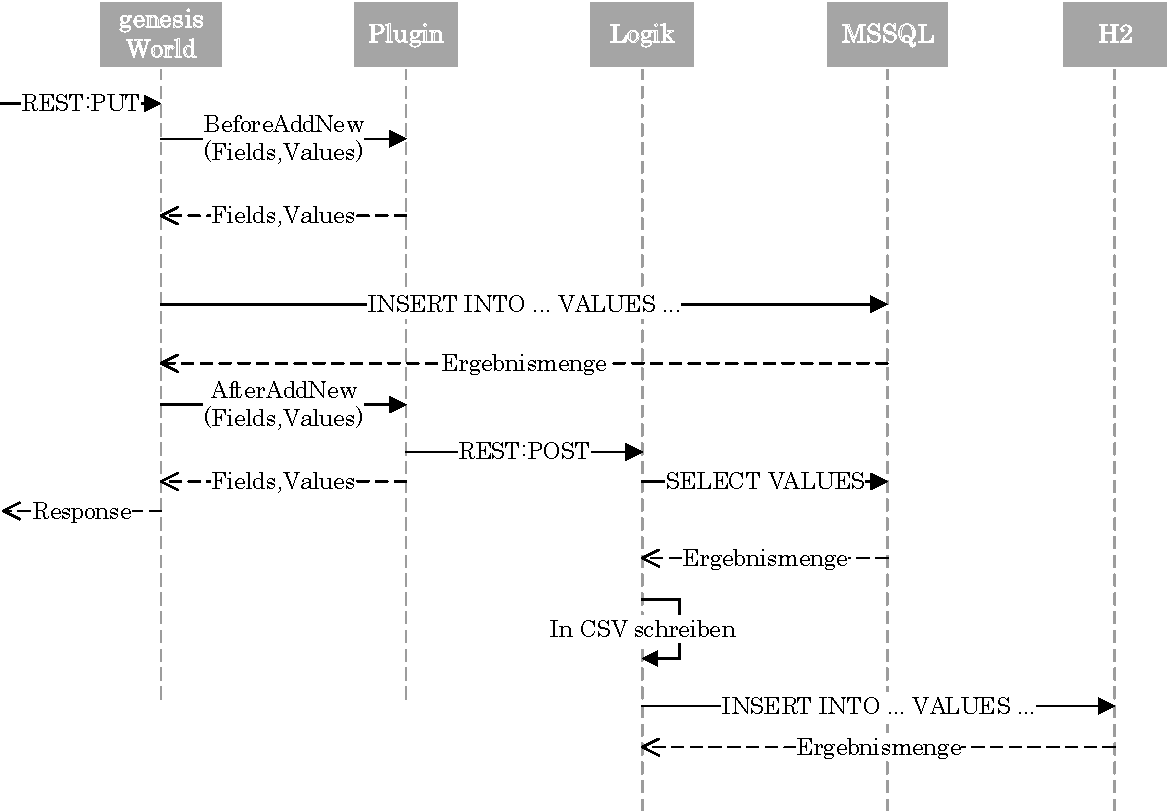
\includegraphics[width=0.8\textwidth]{pics/sequenzdiagramm.pdf}
\caption{Sequenzdiagramm für einen neuen Datensatz}
\label{umsetzung_sequenz}
\end{figure}

In der Methode \textit{AfterAddNew()} des Plugins wird ein Ablauf angestoßen. Indessen wird zuerst überprüft ob der Datensatz eine Relevanz für das System besitzt. Falls er sich als relevant herausstellt, wird die \textit{aGGUID} in einen String konvertiert. Anschließend werden die Header-Werte der \textit{idHttp} Variable gesetzt. Sie beinhalten Werte, wie die URI oder HTTP-Metadaten. Sobald alle Daten in der \textit{idHttp} gesetzt sind, wird ein POST-Request an das Server-Webprojekt im Tomcat-Server übermittelt. 

Der POST-Request enthält die \textit{GGUID} und die Art der Operation, die auf den Daten ausgeführt wurde. Bei neuen Daten beispielsweise wird ein Header namens "newGGUID" mit der zuvor konvertierten \textit{GGUID} als Wert gesetzt. Im Server-Webprojekt wird der neue Wert zuerst in eine CSV-Datei geschrieben und anschließend in die H2-Datenbank eingefügt.


%% ===========================
\section{Oberfläche}
%% ===========================

In diesem Abschnitt wird die Umsetzung der Benutzeroberfläche erörtert. Den Einstiegspunkt für Benutzer stellt das in Abbildung \ref{ergebniss_oberflaeche_anmeld} zu sehende Anmeldefenster dar. Der Hintergrund der Webseite ist in einem dunklen grau gestaltet, um einen Kontrast zum weißen Hintergrund der Bedienelemente zu schaffen. Zur Identifikation des Systems mit der Firma ist das Logo der CAS Software AG im linken Teil abgebildet. Im rechten Teil des Fensters existieren drei Eingabefelder. Zuerst ein Feld zur Eingabe der IP-Adresse des Servers. Die dazugehörige Portnummer wird im darauf folgenden Feld eingegeben. Das dritte Feld ist für den Namen des Nutzers vorgesehen, der den Ausgangspunkt der Analyse darstellt. Abschließend wird ganz klassisch ein Button zum Fortfahren auf der Webseite eingesetzt. Falls allerdings der eingegeben Nutzername nicht existiert, wird eine Warnmeldung direkt über dem zweiten Eingabefeld ausgegeben und auf der Anmeldeseite verblieben. 

\begin{figure}[htbp]
\centering
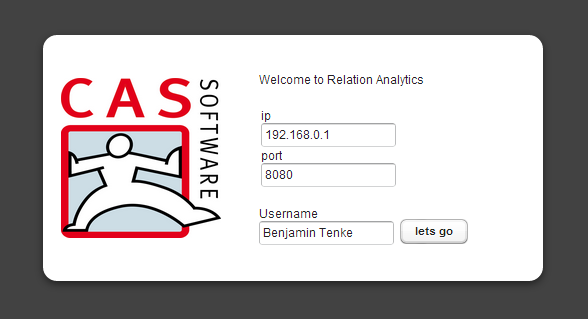
\includegraphics[scale=2.0]{pics/login.png}
\caption{Anmeldefenster}
\label{ergebniss_oberflaeche_anmeld}
\end{figure}

Das Hauptfenster wurde wie in der Abbildung \ref{ergebniss_oberflaeche_haupt} zu sehen umgesetzt. Im oberen Bereich befindet sich eine Leiste, die anhand der Microsoft Richtlinien für Design entworfen wurde. Dies schafft ein vertrautes Gefühl mit der Oberfläche und schafft eine schnelle Akzeptanz bei den Nutzern. Die Leiste ist in vier Bereiche aufgeteilt. Der erste Bereich, ganz links, dient der Gewichtung der CRM-Objekte und dem anstoßen der Abfrage. Aufgrund der Gewichtung in Prozent, ist ein fester Wertebereich von 0 bis 100 vorgegeben. Textfelder eignen sich daher weniger, da sie beliebige Eingaben ermöglichen. Der Einsatz von Reglern bietet eine einfachere und selbsterklärende Form der Bedienung. Der begrenzte und kleine Wertebereich begünstigen den Einsatz der Regler. Zum Stellen der Anfrage wird ein einfacher Button eingesetzt. Direkt unter dem Button befindet sich ein Text, der die benötigte Zeit für die Verarbeitung der Abfrage anzeigt. 

Der zweite Bereich dient zeitlichen Anpassungen. Das erste und dritte Feld können zum Verändern des Betrachtungszeitraums verwendet werden. Sie beinhalten den Anfangs- und Endzeitpunkt. Die manuelle Eingabe des Datums weist eine schlechte Bedienbarkeit auf und ist fehleranfällig, weswegen ein sogenannter "Datumspicker" eingesetzt wird. Dieser befindet sich direkt neben dem Textfeld und öffnet sich nach einem Klick auf das Symbol. Er stellt einen grafischen Kalender dar, aus dem durch klicken auf ein Tag das Datum bestimmt werden kann. Die Möglichkeit zur Eingabe durch direktes Ändern des Textes bleibt allerdings weiterhin erhalten. Die anderen beiden Felder sind für die Gewichtung der Zeit vorgesehen. Diese Felder dienen zur Festlegung von $t_1$ und $t_2$, aus der Abbildung \ref{fig:umsetzung:gewichtungderzeit}. Das obere Feld ist für $t_1$. Hier kann die Zeitspanne zwischen $t_{s}$ und $t_1$ in Tagen festgelegt werden. Der Wert für die Zeitspanne zwischen $t_{e}$ und $t_2$ wird aus dem unteren Eingabefeld entnommen.

Bis auf den Ausschluss von Personen anhand ihrer Gruppen sind alle anderen Kriterien zur Filterungen der Personen im dritten Bereich vorhanden. Mithilfe der Checkboxen kann der Nutzer festlegen, welche Kriterien zum Ausschluss auf die Analyse angewendet werden sollten. Neben der Filterung durch bestimmte Personen, Länder, Städte usw. ist hier eine Begrenzung der Ergebnismenge umgesetzt. Im untersten Feld kann der Benutzer die Anzahl der angezeigten Personen bestimmen.

Der Bereich ganz rechts in der Leiste, ist für den Ausschluss von Gruppen vorgesehen. In ihr werden alle Gruppen im System mit einer Checkbox und einem Namen dargestellt. Dabei können beliebig viele Gruppen ausgewählt werden. Da die Anzahl der Gruppen überschaubar ist, entschied man sich alle anzuzeigen, anstatt einer manuellen Eingabe durch den Nutzer. Dadurch können Benutzer Gruppen auswählen, die sie zuvor nicht beim Namen kannten.

\begin{figure}[htbp]
\centering
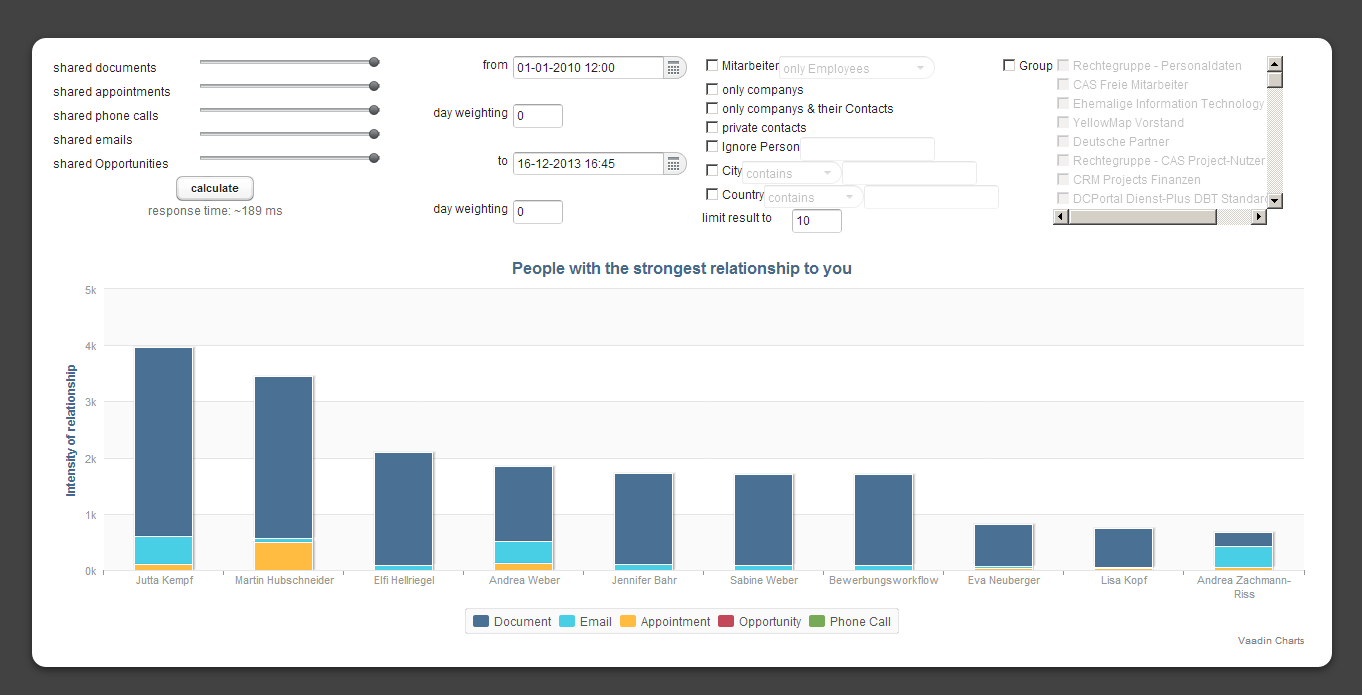
\includegraphics[width=\textwidth]{pics/final_screen.png}
\caption{Hauptseite der Anwendung}
\label{ergebniss_oberflaeche_haupt}
\end{figure}

Den zentralen Bereich des Fensters stellt das Diagramm dar. Die Balken selbst sind in fünf verschiedene Elemente unterteilt. Jedes Element wird durch eine andere Farbe dargestellt. Die fünf Elemente sind die verschiedenen CRM-Objekte. Die Zuordnung der Farbe zu dem jeweiligen Element, wird über eine Legende im unteren Bereich des Fensters umgesetzt. Eine Besonderheit ist, dass durch einen Klick auf eine der Farben, das jeweilige Element von der Darstellung ausgeschlossen wird. Beispielsweise kann der Nutzer auf die blaue Farbe klicken, was einen Neuaufbau des Diagramms ohne Dokumente bewirkt. Durch den Ausschluss wird allerdings keine neue Abfrage gesendet. Das  bedeutet die Reihenfolge in der die Personen angezeigt werden und die Datenbasis bleibt gleich. Mit einem wiederholten Klick auf die entsprechende Farbe in der Legende lässt sich der Originalzustand wiederherstellen. Außerdem kann der Wert eines Balkenteilstücks im Verhältnis zum Gesamtwert des Balkens betrachtet werden. Dies geschieht durch einfaches platzieren des Mauszeigers, auf dem jeweiligen Bereich des Balkens. Dadurch öffnet sich ein Tooltip mit den entsprechenden Informationen.

Die Ausführung der Anfrage erfolgt in der Regel mit dem dafür vorgesehen Button. Die Regler für die Gewichtung der CRM-Objekte und das Datum, jedoch lösen bei Veränderungen automatisch eine neue Abfrage aus. Dies soll die kurze Antwortzeit des Systems untermalen und eine bessere Nutzererfahrung schaffen.

